\documentclass[twoside]{article}
\usepackage[a4paper, bottom=85pt, left=1.85cm, right=1.85cm]{geometry}
\usepackage{fancyhdr}
\usepackage{amsmath}
\usepackage{hyperref}
\usepackage{blindtext}
\usepackage{graphicx}
\graphicspath{{./images/}}
\usepackage[
backend=biber,
citestyle=numeric, 
bibstyle=numeric,
sorting=ynt
]{biblatex}

\addbibresource{konyvek.bib}
\addbibresource{cikkek.bib}

\title{Memrisztorok}
\author{Baranyi Szabolcs, Gyimesi Dávid}
\date{\today}
\renewcommand*\contentsname{Tartalom}
\pagestyle{fancy}
\fancyhead[RO,LE]{BME Villamosmérnöki és Informatikai Kar}

\begin{document}

\maketitle\thispagestyle{fancy}
\begin{abstract}
	\blindtext[5]
\end{abstract}
\pagebreak
\tableofcontents
\newpage
\section{Bevezetés}
A memrisztor története 1971-ben kezdődött, L. Chua\cite{chua} munkájával, amely az alkatrész elméleti alapjait, lehetőségeit, alapvető kérdéskörét fektette le. Komolyabb gyakorlati felhasználások/alkalmazások csak a 2000-es évek elején terjedtek el, a non-volatile (nem felejtő) memóriák általános fejlődésével, és a resistive switching technológia kutatásával. Ezen az alkalmazásterületen a rezisztív alapú (memrisztort megvalósító) nem-felejtő memóriákat ReRAM-nak nevezik. Melletük még szintén kiterjedt kutatásterület a phase-change memóriák, a magnetorezisztív memóriák, vagy például a ferroelektromos memóriák.  \cite{emerging2017}
\section{Kidolgozási módszerek, megjegyzések}
\section{Bibliometriai elemzés, kutatási trendek}
\section{Memrisztorok elméleti összefoglalása, modellezés}
A memrisztor egy olyan ideális hálózati alkatrész, amely karakterisztikája a töltés és a fluxus között értelmezett, így kiteljesíti a négy mennyiség (áram, feszültség, töltés, fluxus) közötti hálózatelméleti négyszöget.\cite{chua} A karakteriszikája (fluxusvezérelt memrisztor): \[d\phi(q) = M(q)dq\]. Tehát fennáll a $v(t) = M(q(t))i(t)$, ilyenkor M a memrisztancia elnevezést kapja, mert mivel az $q(t) = \int_{0}^{t} i(t)dt$, ezért M az áram "múltjától" is függ q(t)-n keresztül. Ugyan, megfigyelve lényegében nemlineáris ellenállásként viselkedik. Az ideális memrisztor megvalósítása eddig nem volt lehetséges, bár tulajdonságai bizonyos alkatrészek/rendszerek (pl. Chua által ajánlott mutátor hálózatok) alkalmazásával közelíthetők. A memrisztor passzivitásához az szükséges, hogy $\int_{-\infty}^{t} p(\tau)d\tau > 0$ teljesüljön bármely t-re, amit a $M(q) > 0 \;\; \forall q$ biztosít. Vagyis, egy, a teljes értelmezési tartományán monoton növő $\phi-q$ görbe mellett a memrisztor passzív alkatrészként viselkedik, tehát kikapcsolás után is megtartja a memrisztancia értékét. Ezáltal, nem-felejtő memóriaként alkalmazható. Tellini et al. szerint \cite{tellini2021} a memrisztor nem egy negyedik független áramköri elem, hanem az idő-variáns ellenállás általánosítása. Ezek mellett, miután Chua és Kang általánosította a dinamikus memrisztív rendszerek fogalmát \cite{chuakang1976}: \begin{align*}\dot{x} &= \vec{f}(\vec{x}, u, t) \\ y &= g(\vec{x}, u, t)u\end{align*} Ez lehetővé tette egyéb memrisztív kialakítások kutatását, például a memkapacitás $q = C(\vec{x}, v, t)v$, vagy a meminduktancia $\varphi = L(\vec{x}, i, t)t$ esetét. Már Mauro et al. is kutattak memrisztív rendszert, az ún. termrisztort \cite{mauro1961}\cite{chuakang1976}\cite{tellini2021}, amely esetén az "idő-variáns rezisztancia" állapotváltozója a hőmérséklet (rendellenes reaktáns komponens az impedanciában, hagyományos dinamikus komponensek nélkül). Ebben az esetben a teljes generált energia megegyezik a disszipált és a tárolt hő összegével $p(t) = v(t)i(t) = \delta(T-T_0) + C\frac{dT}{dt}$ de, memrisztoros rendszer lévén \cite{chuakang1976} szerint $v = R_0(T_0)\exp{\left[\beta\left(\frac{1}{T}-\frac{1}{T_0}\right)\right]i}$
\section{Non-volatile memóriák}
\subsection{Nemfelejtő memóriák bemutatása}
\subsection{Az anyagtudomány szerepe, TiO$_2$, SrTiO$_3$}
A nemfelejtő ReRAM technológia kutatása 2008-ban, a TiO$_2$ (titán-dioxid) fém-szigetelő-fém kialakítás sikerének köszönhetően nagyobb népszerűségre tett szert. A ReRAM lényege, hogy a szigetelő anyagban feszültség hatására dinamikusan egy magas rezisztanciás (HRS), és egy alacsony rezisztanciás (LRS) állapot között váltunk a megfelelő bit írásának megfelelően. Ilyenkor a szigetelőben egy vezető csatorna keletkezik (főként a szennyeződéseknek és az esetleges adalékolt pozitív oxigénionok hatására). Használnak még pl. cink-oxidokat, nikkel-oxidot\cite{emerging2017} vagy stroncium-titanátot (SrTiO$_3$). A legtöbbet kutatott, titán-dioxid alapú memrisztor két darab platinum elektródból, illetve egy közöttük lévő TiO$_2$ rétegből áll. Ez utóbbi egy rendkívül vezetőképes, csökkentett oxigénkoncentrációjú rétegből (TiO$_{2-x}$), és egy kémiailag tökéletes titán-dioxid szegmensből áll. A "szennyezett" TiO2 és a pozitív elektród közötti távolság w. A két elektródra kapcsolt pozitív feszültség hatására a szennyezett titán-dioxid ionjai sodródni kezdenek a pozitív elektród felé, így a w távolság csökken. A konstrukción átfolyó teljes áram a w vastagságú oxidréteg áthatolásától függ, ami rendkívül nemlineáris módon függ a w távolság nagyságától \cite{kolka2015}. Egy ilyen kialakítás dinamikus modellezésében például a w, mint állapotváltozó szerint írható fel az állapotváltozós leírás\cite{pickett2009}. Pickett et al. egy TiO$_2$ crosspoint kialakítást vizsgálták, ahol az egyes cellák esetén a "bipoláris átkapcsolás" jelenségét az ionsodródási sebesség exponenciális függvényében, illetve a sodródási és a diffúziós hatások kölcsönhatásának vonatkozásában modellezték. A két platinum elektród közé a titán-dioxidot katódporlasztással növesztették 250 C-on, O-Ti: $2.00 \pm 0.01$ sztöchiometrikus arányban.
\begin{figure}[h]
\centering
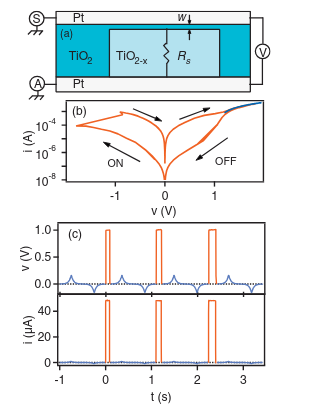
\includegraphics{pickett}
\caption{Pickett et al. fém-szigetelő-fém kialakítása, a szennyezett rutil réteg ellenállása $R_s$, egyéb cuccok\cite{pickett2009}}
\end{figure}
A TiO$_{2-x}$ részt ún. elektroformálással hozták létre, ami az oxidban oxigén vakanciákat hozott létre, ezzel visszafordíthatatlanul lecsökkentve (nagyságrendekkel) az ellenállását. A folyamat önmagába véve annyit takar, hogy 0V-ról +6V-ra rövidrezárták a memrisztort (5 ms kb). Pickett et al. állapotegyenlete a Simmons-csatorna vastagságára (w) a csatornaáramra ($i_M$) nézve erősen nemlineáris összefüggés, mindkét csatornaáram-irány szempontjából.\\
A bipoláris átkapcsolású memrisztív rendszerek alapvető tulajdonsága egyfajta hiszterézis az i-v görbén. Ez teszi lehetővé a "diszkrét" állapotok definiálhatóságát. Bár, a memrisztorok klasszikus értelmezésében is, váltakozóáramú gerjesztésre a i-v karakterisztika az origóban "összefogott" Lissajous-görbéket mutat\cite{chuakang1976}. Ennek oka, hogy a klasszikus értelmezésben a memrisztív rendszerek nem képesek energia tárolására. Ugyan, a gerjesztés frekvenciától függ a görbe "befogott területe", végtelen frekvencia esetén a "hiszteretikus" görbe helyett egyetlen összefüggő görbe lesz. \\
Strukov et al. a titán-dioxid ReRAM kialakítást két sorba kapcsolt ellenállásként értelmezi. \cite{strukov2008} Állapotváltozónak a w-t használták, ami náluk a szennyezett réteg hossza. \begin{align*}
	v(t) &= \left(\mathcal{R}_{ON}\frac{w(t)}{D} + \mathcal{R}_{OFF}\left(1 - \frac{w(t)}{D}\right)\right)i(t) \\
	\frac{dw}{dt} &= \mu_v \frac{\mathcal{R}_{ON}}{D} i(t)
\end{align*}
Tehát a rendszer modellezett memrisztanciája (ha $\mathcal{R}_{ON} \ll \mathcal{R}_{OFF}$): \[
	M(q) = \mathcal{R}_{OFF} \left(1- \frac{\mu_v \mathcal{R}_{ON}}{D^2}q(t)\right)
\]
Soni et al. ezt a modellt nevezi "lineáris ionsodródási modellnek"\cite{soni2022}. Nemlineáris ionsodródási modellek során az állapotváltozó kifejezéséhez egy extra $f(x)$ tényezőt is hozzárendelnek, így az állapotváltozó saját magára is kihat, ezáltal a szennyezett oxidréteg feszültségmenti növekedésének mértékére közvetlenül megadhatunk egy nemlineáris "ablakozó" függvényt.\\
\begin{figure}[h]
	\[ F_p(x) = 1 - (2x - 1)^{2p}\]
	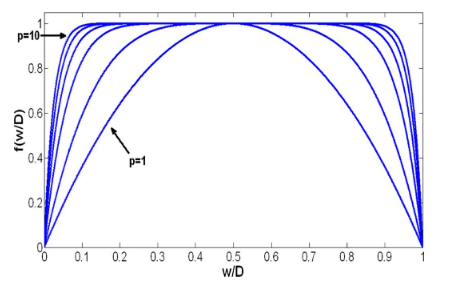
\includegraphics{joglekar}
	\centering
	\caption{Joglekar-féle ablakfüggvény\cite{joglekar2009}\cite{kvatinsky2013}}
\end{figure}

A Pickett-Simmons állapotegyenlet egyszerűbb megadását biztosítja a TEAM modell (ThrEshold Adaptive Memristor)\cite{kvatinsky2013}

Az RS (resistive switching) technológiához szükséges szigetelők kristálytani, szennyezettségi követelményeit, növesztési technológiáit, belső folyamatait és energiaviszonyait \cite{szot2014} részletezi.

\subsection{MIM ReRAM modellezése}
\subsubsection{SPICE modellezés}
Számítógépes SPICE-alapú modellezés a nemlineáris ionsodródási modell alapján.
\[
	R(x) = R_{on}x + R_{off}(1-x)
\]
és $\frac{dx}{dt} = kW(x)I$ ahol pl. $W(x) = 1- (2x-1)^{2p}$. Így pl. $p=1$ mellett $\frac{1}{4}\ln\frac{x}{1-x} = k(q(t) +q_0)$, tehát \[
R(q(t)) = R_{off} + \frac{R_{on}-R_{off}}{ae^{-4kq(t)} + 1}
\] ahol $a = \frac{R_{ini} - R_{off}}{R_{off}-R_{ini}}$
\begin{figure}
	\centering
	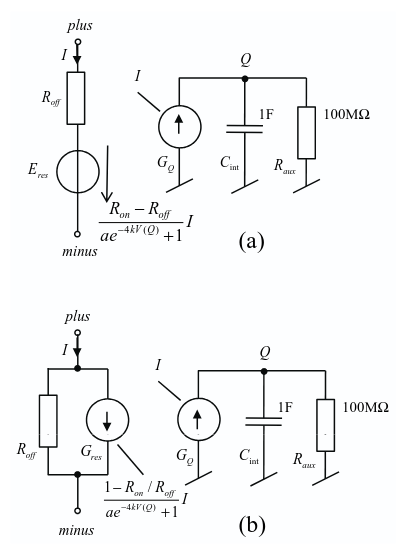
\includegraphics{spice}
	\caption{Lehetséges SPICE megvalósítások\cite{biolek2013}}
\end{figure}
\subsubsection{Verilog-A modellezés alapjai}
\cite{reramva}
\subsection{Verilog-A demó}
\section{3D XPoint}
A 3D XPoint egy crossbar PCM-alapú struktúra, amit az Intel és a Micron Technology dolgozott ki kb. 2008 és 2017 között. Ezen technológiát felhasználó alkatrészek/eszközök 2022. júliusig voltak kaphatók a piacon, Optane (Intel) néven.  PCM (phase-change memory) lévén egy kalkogenid anyag fázisállapotainak kapcsolásával alakítható kis egy HRS és egy LRS állapot. Itt a kalkogenid anyag bizonyos félfémekből, illetve tellúriumból (Te) áll. A teljes félfémes ötvözet ebben az esetben a leggyakoribb, 2:2:5 sztöchiometriai arányú Ge2Sb2Te5, röviden GST. A phase-change memory alapja, hogy különböző nagyságú és idejű áramimpulzusokkal az anyagot egy kristályos, és egy rendezetlen amorf állapot között kapcsoljuk. Az amorf állapot inkább szigetelő (pl. üveg), a kristályos állapot inkább vezető. Amorf állapotban egy $V_th$ határfeszültség alatt szinte egyáltalán nem vezet. Ezt túllépve az anyag rezisztív tulajdonságú lesz, disszipálni kezd. Ha kb. 350 C-ot elér, még nem olvad meg, viszont a részecskék növekedett kinetikus energiája miatt elkezd kristályosodni (ha a SET áramot kb 100ns ideig fenntartjuk). A kristályos állapot energiamentes állapotban is megmarad (ettől lesz a PCM nem-felejtő memória). Ebben az állapotban az anyag kis ellenállású (LRS állapot), ezt egy rövid, alacsony impulzussal olvashatjuk. Az amorf állapotba kapcsolás magasabb  teljesítményen történik (kb. 610 C-ra melegszik a kalkogenid), az anyag megolvad, de az impulzus kis időtartama miatt nincs elég ideje kristályosodni. Ezáltal amorf állapotban szilárdul meg. Ilyenkor az ellenállás sokkal nagyobb ($V_th$ alatt), így ezt is egy rövid impulzussal olvashatjuk. A LRS és a HRS állapot $V_{th}$ alatt egyértelműen megkülönböztethető. \\
\begin{figure}[h]
	\centering
	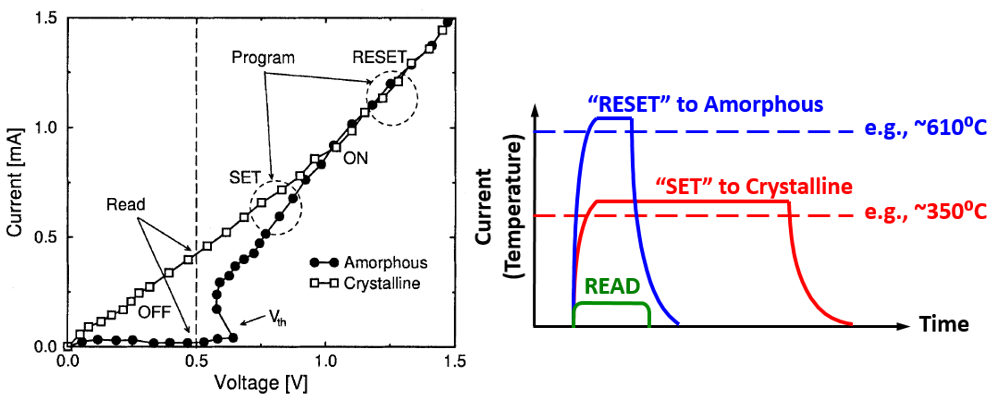
\includegraphics[scale=0.6]{pcm}
	\caption{Amorf és kristályos állapot rezisztív tulajdonságai (1), illetve író-és olvasóimpulzusok (2)\cite{3dxpoint}}
\end{figure}
A 3D XPoint alapja, hogy PCM cellákkal a DRAM-nál sokkal nagyobb cellasűrűség érhető el, illetve a cellakiválasztást nem tranzisztor/dióda, hanem az ún. ovonic threshold switch (OTS) \cite{3dxpoint} valósítja meg. Ez hasonló kalkogenid ötvözetből készül, mint maga a PCM, viszont pl. arzénnel adalékolják, hogy megakadályozzák az anyag kristályosodását (nem állhat be egy "SET" állapotba, így sosem lesz non-volatile kis rezisztanciája), így lehetővé tegyék hogy memória helyett úgy viselkedjen, mint egy "kapcsoló", azaz csak megadott threshold feszültség felett vezessen (konstans amorf állapot). A 2017-es állapot szerint a 3D XPoint technológia 2 ilyen cellaréteget (WL + cella + BL) tartalmaz, ami együtt is sokkal keskenyebb mint az alatta lévő CMOS kontroll hálózat. Guy Blalock, a IM Flash Technologies társelnök-vezérigazgatója 2016-ban egy interjúban azt mondta, elképzelhető 4 réteg is, illetve a dizájn további zsugorításának csökkentéséből fakadó egyéb előnyök, amint az EUV litográfia technológia megérik. \cite{3dxpoint2} A rétegzést nem is a fizikai kiterjedés korlátozza, hanem (tekintve hogy az OFF állapotú OTS-nek sem végtelen az ellenállása) a párhuzamos "káros" áramok mennyisége (nem léphet át egy határt, hogy ne roncsolja a környező cellák értékét, mint pl. a NAND flash esetén $\rightarrow$ "read disturb"). A NAND tárolók esetén általában az egyszerre végrehajtható olvasási ciklusok számát korlázották emiatt. Ezek mellett, a 3D XPoint törlés nélkül programozható (felülírható), a NAND Flash-sel szemben. \\
Az Intel Optane SSD-k bájt-címkézhetők, míg a NAND Flash SSD-k csak page-címkézhetők. Az utóbbiak esetén ezáltal az I/O operációk csak page-ként végezhetők el, így pl. a subpage írás esetén az ún. read-modify-write folyamat szükséges. \cite{yang2020}
A 3D XPoint SSD-ben overwrite melletti írási statisztikák szerint a -- NAND tárolóval szembeni -- helyi felülírási képességnek köszönhetően nincs beépített írás-menti garbage collection, ami élesen csökkentené (kb. 19\%-kal) az írási sebességet/sávszélességet. Így az Optane SSD teljes tár esetén is közel ugyanolyan teljesítményt nyújt (0.5\% körüli hiba), mint normál állapotban. \cite{yang2020}
\section{ReRAM gyakorlati alkalmazásai}
\subsection{Neurális hálózatok, gépi tanulás}
Memrisztorok egyik legelterjedtebb alkalmazása: ANN gyorsítás, pl. crosspoint struktúrával gyors mátrixszámítás, gyorsított regresszió, döntési fák, stb. Belső sztochaszticitásnak köszönhetően probabilisztikus számítások, kombinatorikus optimizáció stb. \cite{jiang2025}
\\
Neuromorfikus chipek \cite{souto2024}

\section{Cutting-edge kutatási területek}

\newpage
\printbibliography[heading=bibintoc, title={Hivatkozások}]


\end{document}
